\section{The Transient model}
\subsection{Package \texttt{it.unibo.kaktor.model}}

As we have already said, the \textit{transient} model consists in a series of entities that represent the description of the actor system that the application designer want to define.
In a first approximation these entities will then be wrapped into \texttt{ActorBasic} instances that will be used as regular.

We remember that the main entities defined into the \texttt{QA-System} are:
\begin{itemize}
	\item \textbf{actors} active components that are able to receive messages and handle them in a proper way;
	\item \textbf{body} as the main behavior of each actor;
	\item \textbf{messages} as the communication unit for the actors;
	\item \textbf{states} (for finite state machine actors);
	\item \textbf{transitions} (for finite state machine actors);
	\item \textbf{contexts};
\end{itemize}

\begin{figure}[h!]
	\centering
	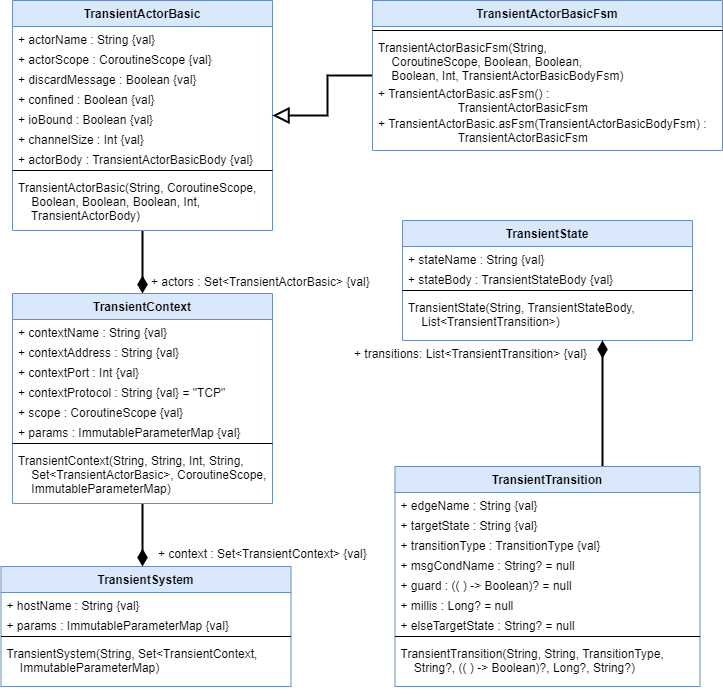
\includegraphics[width=\textwidth]{img/[UML]it.unibo.kaktor.model}
	\caption{UML diagram for the Transient Model}
	\label{fig::uml_model}
\end{figure}

Slightly abusing the \texttt{UML} notation, the figure \ref{fig::uml_model} shows the diagram of the transient model package. We have provided these classes:
\begin{itemize}
	\item \href{https://github.com/LM-96/QA-Extensions/blob/main/it.unibo.qakactor/src/main/kotlin/model/TransientActorBasic.kt}{\underline{\textbf{\texttt{TransientActorBasic}}}}:\\
	The class represents the description of an actor (e.g. its name, its scope, its channel size and other options), particularly \textbf{its body} that will be described in a few lines; this is the central class of the model that will be \textit{wrapped} into the \texttt{ActorBasic} class used from the system for the runtime implementation.
	
	\item \href{https://github.com/LM-96/QA-Extensions/blob/main/it.unibo.qakactor/src/main/kotlin/model/TransientActorBasicFsm.kt}{\underline{\textbf{\texttt{TransientActorBasicFsm}}}}:\\
	This class represents the description of an actor that is a \textit{finite state machine}. So it extends the \texttt{TransientActorBasic} class but has a \textit{finite state body} instead of the normal body of its super-class.
	
	\item
	\href{https://github.com/LM-96/QA-Extensions/blob/main/it.unibo.qakactor/src/main/kotlin/model/TransientState.kt}{\underline{\textbf{\texttt{TransientState}}}}:\\
	This class represents the description of a state of a finite state machine actor. It has a 	\textit{name} and a \textit{state body} that will be called when a \textit{FSM} actor enters the state.
	
	\item
	\href{https://github.com/LM-96/QA-Extensions/blob/main/it.unibo.qakactor/src/main/kotlin/model/TransitentTransition.kt}{\underline{\textbf{\texttt{TransientTransition}}}}:\\
	This class represents the description of a transition from one state to another into a \textit{FSM} actor. So it has an \textit{edge name} used to identify uniquely the transition, a \textit{target state} and a \textit{type}. Based on the type it also has additional fields used be the specific type.
	
	\item 
	\href{https://github.com/LM-96/QA-Extensions/blob/main/it.unibo.qakactor/src/main/kotlin/model/TransientContext.kt}{\underline{\textbf{\texttt{TransientContext}}}}:\\
	This class represents the description of a context that contains a collection of actors. In addition to this, a context also have some field that describes some of its characteristics (like its name, its address and so on).
	
	\item 
	\href{https://github.com/LM-96/QA-Extensions/blob/main/it.unibo.qakactor/src/main/kotlin/model/TransientSystem.kt}{\underline{\textbf{\texttt{TransientSystem}}}}:\\
	This class represents the description of the entire system that will be executed. As a \texttt{TransientContext} it also has a \texttt{ImmutableParameterMap} that is an object defined in another package that maintains a series of key-object pairs for re-usability.
	\textbf{This is the end class of the \textit{transient model} that will be passed to method that load and build the entire system}.
\end{itemize}

\subsection{Package \texttt{it.unibo.kaktor.model.actorbody}}

We have shown that the \texttt{TransientActorBasic} class maintains an object that represents the actor body. Same for the \texttt{TransientActorBasicFsm} class in which the difference is that the body has the behavior of a finite state machine.

\begin{figure}[h!]
	\centering
	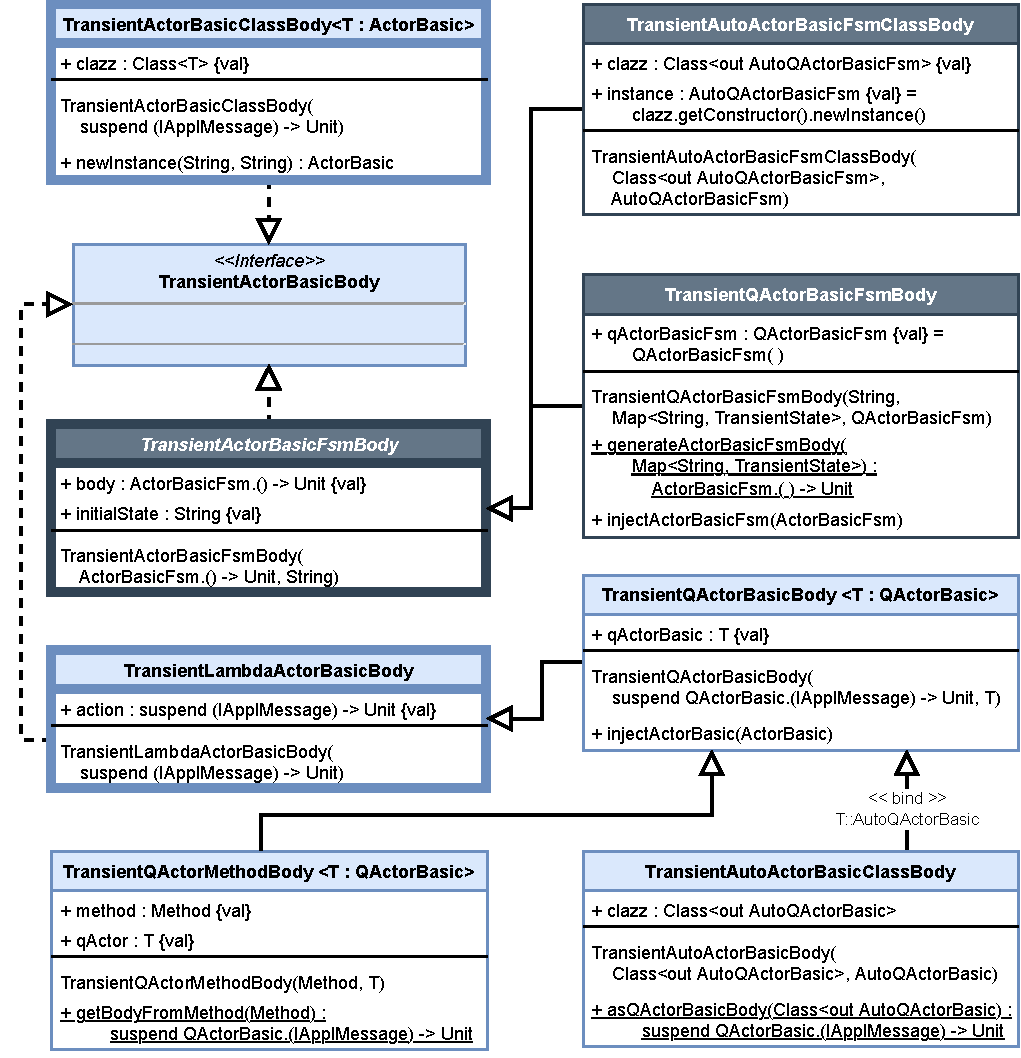
\includegraphics[width=\textwidth]{img/[UML]it.unibo.kaktor.model.actorbody_onlyactorbody}
	\caption{UML diagram for the Transient Model of the actor body}
	\label{fig::uml_model_body}
\end{figure}

The figure \ref{fig::uml_model_body} summarizes the package that contains the class for the actor body. The main classes of this package are:

\begin{itemize}
	\item 	\href{https://github.com/LM-96/QA-Extensions/blob/main/it.unibo.qakactor/src/main/kotlin/model/actorbody/TransientActorBasicBody.kt}{\underline{\textbf{\texttt{TransientActorBasicBody}}}}:\\
	This classes that implements this symbolic interface are actor basic bodies.
	
	\item 	\href{https://github.com/LM-96/QA-Extensions/blob/main/it.unibo.qakactor/src/main/kotlin/model/actorbody/TransientLambdaActorBasicBody.kt}{\underline{\textbf{\texttt{TransientLambdaActorBasicBody}}}}:\\
	This is the main class for a body of an \texttt{ActorBasic} instance. It maintains a \href{https://kotlinlang.org/docs/lambdas.html}{\textit{lambda function}} that describes the actions the actor will have to perform when receives a message.
	
	\item 	\href{https://github.com/LM-96/QA-Extensions/blob/main/it.unibo.qakactor/src/main/kotlin/model/actorbody/TransientActorBasicFsmBody.kt}{\underline{\textbf{\texttt{TransientActorBasicFsmBody}}}}:\\
	This is the main class for a body of an \texttt{ActorBasicFsm} instance. It maintains a \href{https://kotlinlang.org/docs/lambdas.html#closures}{\textit{lambda function with closure}} that contains the actions to be create an instance of the \texttt{ActorBasicFsm} class\footnote{See the official \texttt{QAK} documentations for details about the creation of a finite state machine actor.} and also the name of the initial state.
\end{itemize}

The other classes of this package are useful in order to easily create instances of these main superclasses and will be clarified soon.

\begin{figure}[h!]
	\centering
	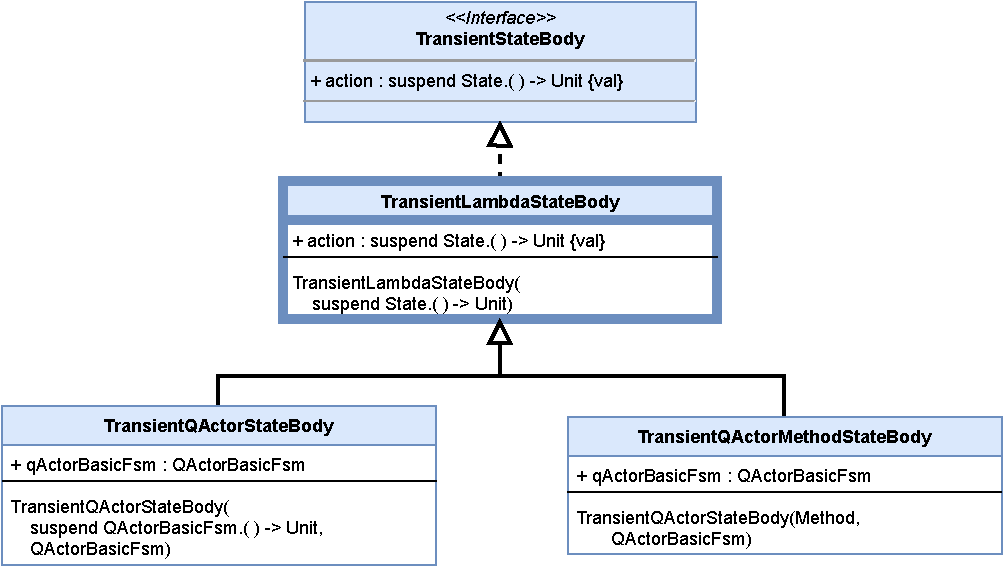
\includegraphics[width=\textwidth]{img/[UML]it.unibo.kaktor.model.actorbody_onlystatebody}
	\caption{UML diagram for the Transient Model of the actor body}
	\label{fig::uml_model_state_body}
\end{figure}

The figure \ref{fig::uml_model_state_body} shows the classes describing the body of a state. It contains:
\begin{itemize}
	\item 	\href{https://github.com/LM-96/QA-Extensions/blob/main/it.unibo.qakactor/src/main/kotlin/model/actorbody/TransientStateBody.kt}{\underline{\textbf{\texttt{TransientStateBody}}}}:\\
	This classes that implements this symbolic interface are finite state machines bodies.
	
	\item 	\href{https://github.com/LM-96/QA-Extensions/blob/main/it.unibo.qakactor/src/main/kotlin/model/actorbody/TransientLambdaStateBody.kt}{\underline{\textbf{\texttt{TransientLambdaStateBody}}}}:\\
	This is the main class for a body of a finite state machine. It maintains a \href{https://kotlinlang.org/docs/lambdas.html}{\textit{lambda function}} that describes the actions the actor will have to perform when enters the state owning this body.
\end{itemize}
The other two subclasses will be used to easily create instance of lambda state body and will be explained in the next sections.




